%!TEX root = SISC_elastic_3d.tex
\subsection{Semi-discretization of the elastic wave equation}\label{semi_discrete_form}

\begin{figure}[htbp]
	\centering
	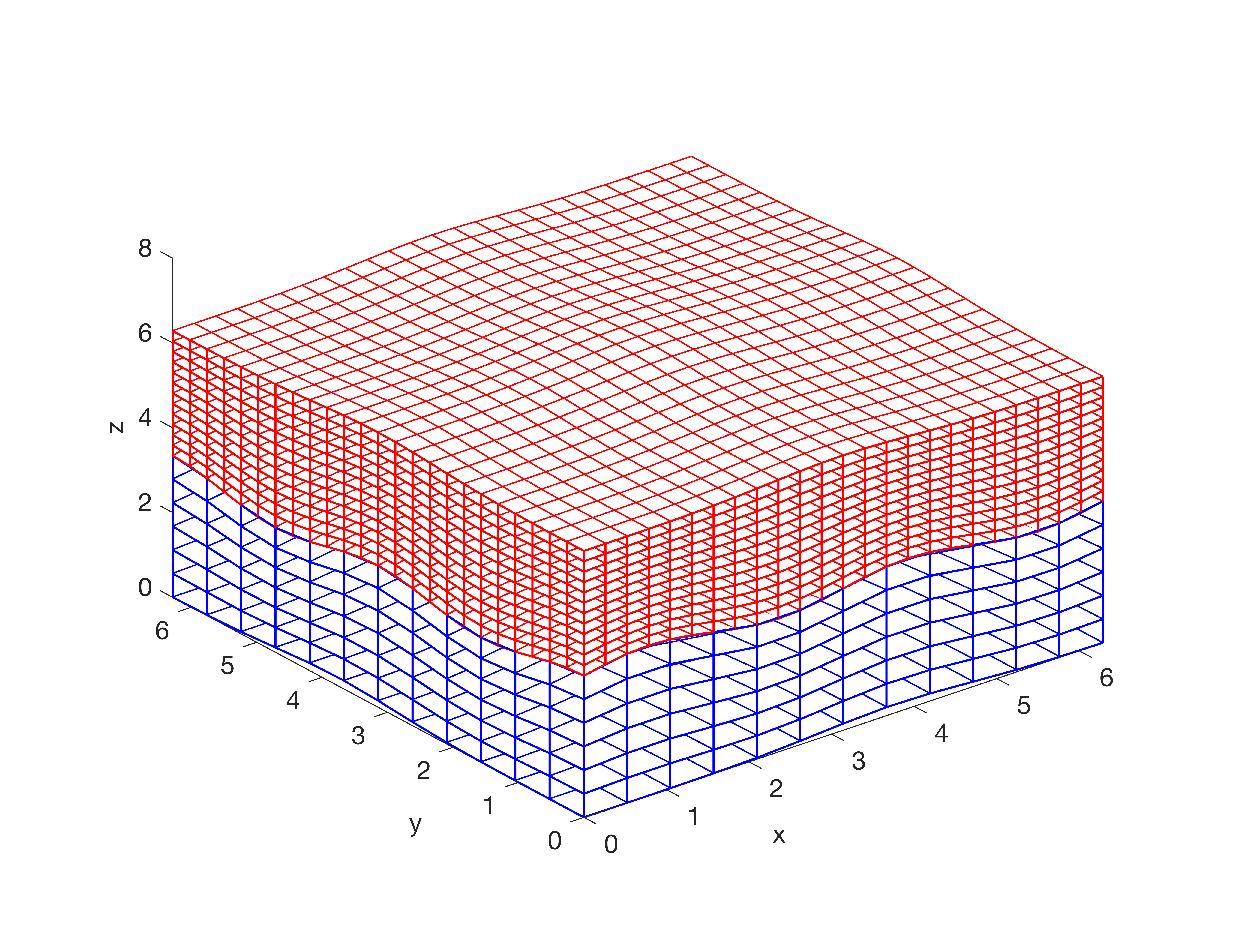
\includegraphics[width=0.6\textwidth,trim={0.4cm 0.7cm 0.8cm 1.4cm}, clip]{physical_discretization.eps}
	\caption{The sketch for the curvilinear mesh of the physical domain $\Omega$. The blue region is the spatial discretization of coarse subdomain $\Omega^c$ and the red region is the spatial discretization of the fine domain $\Omega^f$. Note that $x,y,z$ in the graph correspond to $x^{(1)}, x^{(2)}, x^{(3)}$ respectively. 
	 }\label{physical_discretization}
\end{figure}

In this section, we discretize the elastic wave equations (\ref{elastic_curvi}) and  (\ref{elastic_curvi_f}) with mesh refinement interface $\Gamma$. Without loss of generality, we assume the ratio of mesh sizes in the reference domains is $1:2$, that is the mesh sizes satisfy
\[h_1(n_1^h-1) = 1, \ \ \ h_2(n_2^h-1) = 1, \ \ \ h_3(n_3^h-1) = 1,\]
and
\[2h_1(n_1^{2h}-1) = 1, \ \ \ 2h_2(n_2^{2h}-1) = 1, \ \ \ 2h_3(n_3^{2h}-1) = 1,\]
respectively. Other ratios can be treated analogously. Figure \ref{physical_discretization} gives an illustration of the discretization of a physical domain. This is an ideal mesh if the wave speed in $\Omega^f$ is half of the wave speed in $\Omega^c$.

In seismic wave simulation, far-field boundary conditions are often imposed in the $x^{(1)}$ and $x^{(2)}$ directions. Here, our focus is on the numerical treatment of the interface conditions (\ref{interface_cond}). We assume periodic boundary conditions in $x^{(1)}$ and $x^{(2)}$, and ignore the boundaries in $x^{(3)}$. In Figure \ref{section_discretization}, we fix $x^{(2)} = 0$ and present the $x^{(1)}$-$x^{(3)}$ section of the domain $\Omega$ in both curvilinear space and parameter space.
\begin{figure}[htbp]
	\centering
	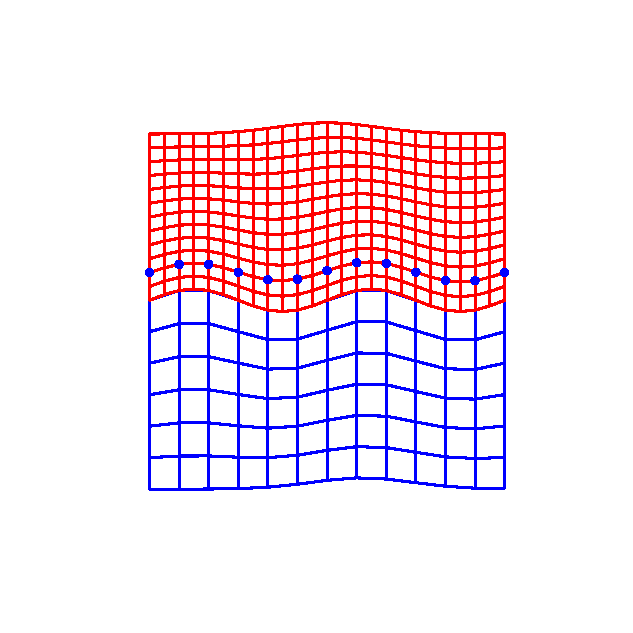
\includegraphics[width=0.45\textwidth,trim={1.0cm 2.0cm 1.0cm 1.8cm}, clip]{physical_section_discretization.eps}
	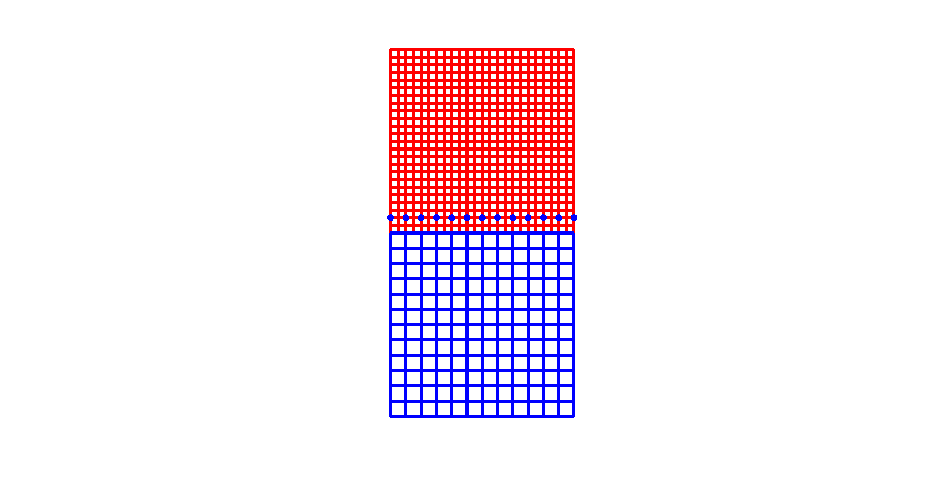
\includegraphics[width=0.45\textwidth,trim={1.0cm 2.0cm 1cm 1.8cm}, clip]{parameter_section_discretization.eps}
	\caption{The sketch of spatial discretization of $x^{(1)}$-$x^{(3)}$ section with $x^{(2)} = 0$. From the left to the right are for physical domain and parameter space, respectively. The blue dots are the ghost points for the coarse domain $\Omega^c$.}\label{section_discretization}
\end{figure}

 To condense notations, we introduce the multi-index notations
\[{\bf i} = (i,j,k),\ \ {\bf r}_{\bf i} = (r^{(1)}_i,r^{(2)}_j,r^{(3)}_k),\ \ {\bf x}^{\{f,c\}}_{\bf i} = (x^{\{f,c\},(1)}_i,x^{\{f,c\},(2)}_j,x^{\{f,c\},(3)}_k),\ \ {\bf x}_{\bf i}^{\{f,c\}} = {\bf X}^{\{f,c\}}({\bf r}_{\bf i}),\]
where $\{\cdot,\cdot\}$ represents the component-wise identities. Note that for ${\bf x}^f_{\bf i}\in\Omega^f$, we have $i\in[1,n_1^h]$, $j\in[1,n_2^h]$, $k\in[1,n_3^h]$; for ${\bf x}^c_{\bf i}\in\Omega^c$, we have $i\in[1,n_1^{2h}]$, $j\in[1,n_2^{2h}]$, $k\in[1,n_3^{2h}]$; for ${\bf x}_{\bf i}^c \in \Gamma\cap\Omega^c$, we have $i\in[1,n_1^{2h}]$, $j\in[1,n_2^{2h}]$, $k = n_3^{2h}$; for ${\bf x}_{\bf i}^f \in \Gamma\cap\Omega^f$, we have $i\in[1,n_1^h]$, $j\in[1,n_2^h]$, $k = 1$; for ${\bf x}_{\bf i}^f\in \Omega \setminus \Omega^c := \overline{\Gamma}$, we have $i\in[1,n_1^h]$, $j\in[1,n_2^h]$, $k\in[2,n_3^h]$. %We want to mention that we have abused the symbol $\bar{\Gamma}$ a little bit to only contain the grid points in $\Omega^f$ but not in $\Omega^c$.
Now, denote the grid functions in $\Omega^f$ and $\Omega^c$ by
\[{\bf f} = ({\bf f}^1, {\bf f}^2, {\bf f}^3)^T\ \ \ \ \mbox{and}\ \ \ \  {\bf c} = ({\bf c}^1, {\bf c}^2, {\bf c}^3)^T,\]
respectively. Here, 
\[{\bf f}^l\approx F_l({\bf r}), \ \ {\bf X}^f({\bf r})\in\Omega^f,\ \ l=1,2,3 ,\]
and
\[{\bf c}^l \approx C_l({\bf r}),\ \ {\bf X}^c({\bf r})\in\Omega^c, \ \ l = 1,2,3.\]
Furthermore, we define ${\bf f}_{\Gamma}$ as the fine grid function for ${\bf X}^f({{\bf r}})\in\Gamma$, ${\bf c}_{\Gamma}$ as the coarse grid function for ${\bf X}^c({{\bf r}})\in\Gamma$ and ${\bf f}_{\overline{\Gamma}}$ as the fine grid function for ${\bf X}^f({{\bf r}})\in\overline{\Gamma}$. Particularly, we define $\wt{\bf c} = (\wt{\bf c}^1,\wt{\bf c}^2,\wt{\bf c}^3)^T$ as the coarse grid function which contains both grids in $\Omega^c$ and ghost points outside $\Omega^c$ with $i\in[1,n_1^{2h}], j\in[1,n_2^{2h}], k\in[0,n_3^{2h}+1]$. Then we approximate the elastic wave equation (\ref{elastic_curvi}) in $\Omega^c$ by
\begin{equation}\label{elastic_semi_c}
{\varrho}^{2h} {\bf c}_{tt} =( \mathcal{ J}^{2h})^{-1}\left(\sum_{l=1}^2\mathcal{G}_l^{2h}({N}_{ll}^{2h}){\bf c}+\wt{\mathcal{G}}_3^{2h}({N}_{33}^{2h}){\wt{\bf c}}+\sum_{l=1}^3\sum_{m=1,m\neq l}^3\mathcal{D}_l^{2h}(\mathcal{N}_{lm}^{2h}\mathcal{D}_m^{2h}{\bf c})\right) := \wt{\mathcal{L}}^{2h} {\wt {\bf c}},
\end{equation}
where 
\begin{align}\label{rho_j}
\varrho^{2h} = \left(\begin{array}{ccc}
{\bm \rho}^{2h}& ~  & ~ \\
~ & {\bm \rho}^{2h} & ~ \\
~ &~  &{\bm \rho}^{2h}\end{array}\right),\ \ \ \mathcal{J}^{2h} = \left(\begin{array}{ccc}
{\bf J}^{2h}& ~  & ~ \\
~ & {\bf J}^{2h} & ~ \\
~ &~  &{\bf J}^{2h}\end{array}\right)
\end{align}
with both ${\bm \rho}^{2h}$ and ${\bf J}^{2h}$ are diagonal matrices of size  $n_1^{2h}n_2^{2h}n_3^{2h}\times n_1^{2h}n_2^{2h}n_3^{2h}$. The diagonal entries of ${\bm \rho}^{2h}$ and ${\bf J}^{2h}$ are values of density function $\rho^c$ and Jacobian of transformation $J^c$ on the grids in $\Omega^c$, respectively.
The operators $\mathcal{G}_l^{2h}({N}_{ll}^{2h})$, $l=1,2$ are defined as
\begin{align}\label{g1122}
\mathcal{G}^{2h}_l({N}_{ll}^{2h}) = \left(\begin{array}{ccc}
Q_l^{2h}(N_{ll}^{2h}(1,1)) & Q_l^{2h}(N_{ll}^{2h}(1,2))  & Q_l^{2h}(N_{ll}^{2h}(1,3)) \\
Q_l^{2h}(N_{ll}^{2h}(2,1)) & Q_l^{2h}(N_{ll}^{2h}(2,2))  & Q_l^{2h}(N_{ll}^{2h}(2,3)) \\
Q_l^{2h}(N_{ll}^{2h}(3,1)) & Q_l^{2h}(N_{ll}^{2h}(3,2))  & Q_l^{2h}(N_{ll}^{2h}(3,3)) \end{array}\right),
\end{align}
where $Q_l^{2h}(N_{ll}^{2h}(i,j))$, $i,j = 1,2,3$, are $n_1^{2h}n_2^{2h}n_3^{2h}\times n_1^{2h}n_2^{2h}n_3^{2h}$ matrices with the central difference stencils in direction $r^{(l)}$ for second derivative with variable coefficient. Here, we also use a matlab notation $N_{ll}^{2h}(i,j)$ to represent the $i'$th row and $j'$th column of matrix $N_{ll}^{2h}$. Note that for each grid point, $N_{ll}^{2h}$ is a $3\times3$ matrix and its values are $N_{ll}^c$ evaluated at the grid points. As for $\wt{\mathcal{G}}_3^{2h}({N}_{33}^{2h})$, it has a structure
\[ \wt{\mathcal{G}}^{2h}_3({N}_{33}^{2h}) = \left(\begin{array}{ccc}
\wt{G}_3^{2h}(N_{33}^{2h}(1,1)) & \wt{G}_3^{2h}(N_{33}^{2h}(1,2))  & \wt{G}_3^{2h}(N_{33}^{2h}(1,3)) \\
\wt{G}_3^{2h}(N_{33}^{2h}(2,1)) & \wt{G}_3^{2h}(N_{33}^{2h}(2,2))  & \wt{G}_3^{2h}(N_{33}^{2h}(2,3)) \\
\wt{G}_3^{2h}(N_{33}^{2h}(3,1)) & \wt{G}_3^{2h}(N_{33}^{2h}(3,2))  & \wt{G}_3^{2h}(N_{33}^{2h}(3,3)) \end{array}\right),\]
where $\wt{G}_3^{2h}(N_{33}^{2h}(i,j))$, $i,j = 1,2,3$, are $n_1^{2h}n_2^{2h}n_3^{2h}\times n_1^{2h}n_2^{2h}(n_3^{2h}+2)$ matrices which are defined as in (\ref{sbp_2nd_1}) for direction $r^{(3)}$. 

Now, let's look at the terms $\mathcal{D}_l^{2h}(\mathcal{N}_{lm}^{2h}\mathcal{D}_m^{2h})$, $l = 1,2,3, m = 1,2,3, l\neq m$. We first explain the cases with $l = 1,2$ and $m = 1,2$ by using $\mathcal{D}_1^{2h}(\mathcal{N}_{12}^{2h}\mathcal{D}_2^{2h})$ as an example. The other cases are analogous. We have 
\begin{equation}\label{D12}
\mathcal{D}_1^{2h} = {\bf I}\otimes D_1^{2h} \otimes {\bf I}_2 \otimes {\bf I}_3,\ \ \ \mathcal{D}_2^{2h} ={\bf I}\otimes {\bf I}_1\otimes D_2^{2h}\otimes {\bf I}_3,
\end{equation}
where ${\bf I}$ is a $3\times3$ identity matrix, ${\bf I}_l$, $l = 1,2,3$ are $n_l^{2h}\times n_l^{2h}$ identity matrices, $D_1^{2h}$ is a $n_1^{2h}\times n_1^{2h}$ matrix with central difference stencil for first order derivative in direction $r^{(1)}$, $D_2^{2h}$ is a matrix of size $n_2^{2h}\times n_2^{2h}$ with central difference operator for first order derivative in direction $r^{(2)}$ as stencil, $\mathcal{N}_{12}^{2h}$ is a $3n_1^{2h}n_2^{2h}n_3^{2h}\times3n_1^{2h}n_2^{2h}n_3^{2h}$ matrix with a structure
\begin{align}\label{N12}
\mathcal{N}_{12}^{2h}= \left(\begin{array}{ccc}
\mathscr{N}_{12}^{2h,11}&\mathscr{N}_{12}^{2h,12}& \mathscr{N}_{12}^{2h,13}\\
\mathscr{N}_{12}^{2h,21} & \mathscr{N}_{12}^{2h,22} & \mathscr{N}_{12}^{2h,23} \\
\mathscr{N}_{12}^{2h,31}&\mathscr{N}_{12}^{2h,32}&  \mathscr{N}_{12}^{2h,33}\\ \end{array}\right),
\end{align}
where $\mathscr{N}_{12}^{2h,ij}$, $i,j = 1,2,3$ are diagonal matrices of size $n_1^{2h}n_2^{2h}n_3^{2h}\times n_1^{2h}n_2^{2h}n_3^{2h}$ with the diagonal values to be $N_{12}^{c}(i,j)$ evaluated at the coarse grid points, i.e., $N_{12}^{2h}(i,j)$. 

Then, let's look at the terms with either $l = 3$ or $m = 3$, we use $\mathcal{D}_1^{2h}(\mathcal{N}_{13}^{2h}\mathcal{D}_3^{2h})$ as an example and the other cases are similar,
\begin{equation}\label{D13}
\mathcal{D}_1^{2h} = {\bf I}\otimes D_1^{2h} \otimes {\bf I}_2 \otimes {\bf I}_3,\ \ \ \mathcal{D}_3^{2h} ={\bf I}\otimes {\bf I}_1\otimes {\bf I}_2\otimes D_3^{2h},
\end{equation}
where $\mathcal{D}_1^{2h}$ is defined in (\ref{D12}) and $D_3^{2h}$ is a matrix of size $n_3^{2h}\times n_3^{2h}$ defined in (\ref{first_sbp}) for direction $r^{(3)}$, $\mathcal{N}_{13}^{2h}$ has a similar definition as $\mathcal{N}_{12}^{2h}$ in (\ref{N12}).

Next, we approximate the elastic wave equation (\ref{elastic_curvi_f}) for the fine grids. We first consider all fine grid points not at the interface, and have the semi-discretization
\begin{equation}\label{elastic_semi_f}
\varrho^h_{\overline{\Gamma}} ({\bf f}_{\overline{\Gamma}})_{tt} =
( \mathcal{ J}_{\overline{\Gamma}}^{h})^{-1}\left(\sum_{l=1}^3\Big(\big(\mathcal{G}_l^{h}({N}_{ll}^h){\bf f}\big)\Big|_{\overline{\Gamma}}+\sum_{m=1,m\neq l}^3\big(\mathcal{D}_l^{h}(\mathcal{N}_{lm}^{h}\mathcal{D}_m^{h}{\bf f})\big)\Big|_{\overline{\Gamma}}\Big)\right) := \mathcal{L}^h{\bf f}\Big|_{\overline{\Gamma}},
\end{equation}
where ${\varrho}^{h}_{\overline{\Gamma}}$ and ${\mathcal{J}}^{h}_{\overline{\Gamma}}$ are $3n_1^hn_2^h(n_3^h-1)\times 3n_1^hn_2^h(n_3^h-1)$ diagonal matrices, which have similar definitions as in (\ref{rho_j}), but correspond to the grids in $\overline{\Gamma}$. In addition, the terms $\mathcal{G}_l^h({N}_{ll}^h), l = 1,2$ and $\mathcal{D}_l^h(\mathcal{N}_{lm}^h\mathcal{D}_m^h), l=1,2,3,m=1,2,3,l\neq m$ in (\ref{elastic_semi_f}) have similar definitions as in (\ref{elastic_semi_c}) but corresponds to the grids in the fine domain $\Omega^f$. And $\mathcal{G}_3^h({N}_{33}^h)$ is defined as
\[ \mathcal{G}^{h}_3({N}_{33}^h) = \left(\begin{array}{ccc}
G_3^{h}(N_{33}^{h}(1,1)) & G_3^{h}(N_{33}^{h}(1,2))  & G_3^{h}(N_{33}^{h}(1,3)) \\
G_3^{h}(N_{33}^{h}(2,1)) & G_3^{h}(N_{33}^{h}(2,2))  & G_3^{h}(N_{33}^{h}(2,3)) \\
G_3^{h}(N_{33}^{h}(3,1)) & G_3^{h}(N_{33}^{h}(3,2))  & G_3^{h}(N_{33}^{h}(3,3)) \end{array}\right),\]
where ${G}_3^{h}(N_{33}^{h}(i,j))$, $i,j = 1,2,3$, are $n_1^{h}n_2^{h}n_3^{h}\times n_1^{h}n_2^{h}n_3^{h}$ matrices which are defined as in (\ref{sbp_2nd_2}) for direction $r^{(3)}$. The symbol $(\cdot)\big|_{\bar{\Gamma}}$ in (\ref{elastic_semi_f}) corresponds to the data in $\bar{\Gamma}$.

For the approximation on the interface $\Gamma$, we obtain the numerical solution by injection using a scaled interpolation operator
\begin{equation}\label{continuous_sol}
{\bf f}_{\Gamma} = \wt{\mathcal{P}}({\bf c}_{\Gamma}),
\end{equation}
which imposes the continuity of the solution at the interface $\Gamma$. 

For energy stability, the operator $ \wt{\mathcal{P}}$ must be in a specific form 
\[\wt{\mathcal{P}} = (\mathcal{J}^h_\Gamma \bm{\Lambda}^h)^{-\frac{1}{2}}\mathcal{P}(\mathcal{J}^{2h}_\Gamma \bm{\Lambda}^{2h})^{\frac{1}{2}}.\]
Here, both  $\mathcal{P}$ and $\bm{\Lambda}^{2h}$ are $3n_1^{2h}n_2^{2h}n_3^{2h}\times 3n_1^{2h}n_2^{2h}n_3^{2h}$ matrices and the size of $\bm{\Lambda}^{h}$ is $3n_1^{h}n_2^{h}n_3^{h}\times 3n_1^{h}n_2^{h}n_3^{h}$. They have the following structures
\begin{align}\label{iandr}
\mathcal{P} = \left(\begin{array}{ccc}
{\bf P}& ~  & ~ \\
~ & {\bf P} & ~ \\
~ &~  &{\bf P}\end{array}\right), \ \ \ 
\bm{\Lambda}^h = \left(\begin{array}{ccc}
\Lambda^h& ~  & ~ \\
~ & \Lambda^h & ~ \\
~ &~  &\Lambda^h\end{array}\right), \ \ \ \bm{\Lambda}^{2h} = \left(\begin{array}{ccc}
\Lambda^{2h}& ~  & ~ \\
~ & \Lambda^{2h} & ~ \\
~ &~  &\Lambda^{2h}\end{array}\right).
\end{align}
The matrix $\bf P$ is of size $n_1^{2h}n_2^{2h}n_3^{2h}\times n_1^{2h}n_2^{2h}n_3^{2h}$. Since the mesh refinement ratio is $1:2$, the stencils of the fourth order accurate interpolation operator ${\bf P}$ in two dimensions have four cases, see the illustration in  Figure \ref{interpolation}. 
The matrix $\Lambda^{h}$ is a $n_1^{h}n_2^{h}n_3^{h}\times n_1^{h}n_2^{h}n_3^{h}$ diagonal matrix and its diagonal values are $|\nabla_x^f r^{(3)}|$ evaluated at the fine grid points at interface $\Gamma$. Similarly, $\Lambda^{2h}$ is a $n_1^{2h}n_2^{2h}n_3^{2h}\times n_1^{2h}n_2^{2h}n_3^{2h}$ diagonal matrix with diagonal values  $|\nabla_x^c r^{(3)}|$ evaluated at the coarse grid points at interface $\Gamma$.

We note that \eqref{continuous_sol} is equivalent to the more complicated form
\begin{equation}\label{elastic_semi_f_i}
{\varrho}^h_\Gamma ({\bf f}_\Gamma)_{tt} =
( {\mathcal{ J}}^{h}_\Gamma)^{-1}\left(\sum_{l=1}^3\Big(\big(\mathcal{G}_l^{h}({N}_{ll}^h){\bf f}\big)\Big|_\Gamma+\sum_{m=1,m\neq l}^3\big(\mathcal{D}_l^{h}(\mathcal{N}_{lm}^{h}\mathcal{D}_m^{h}{\bf f})\big)\Big|_\Gamma\Big) \right) + {\bm \eta} := \mathcal{L}^h{\bf f}\Big|_\Gamma + {\bm \eta},
\end{equation}
with 
\begin{equation}\label{eta}
{\bm \eta} = {\varrho}^h_{\Gamma}\wt{\mathcal{P}}\left(\big(({ \varrho}^{2h})^{-1}\wt{\mathcal{L}}^{2h} \wt{{\bf c}}\big)\Big|_{\Gamma}\right) - \mathcal{L}^{h}{\bf f}\Big|_{\Gamma}.
\end{equation}
Here, ${\varrho}^{h}_{\Gamma}$ and ${\mathcal{ J}}^{h}_{\Gamma}$ are $3n_1^hn_2^h\times 3n_1^hn_2^h$ diagonal matrices with similar definitions as in (\ref{rho_j}) with fine grids at $\Gamma$. The size of the column vector $\big(({\varrho}^{2h})^{-1}\wt{L}^{2h} \wt{{\bf c}}\big)\big|_{\Gamma}$ is $3n_1^{2h} n_2^{2h}$. 

 We note that $\bm \eta$ is approximately zero with a second order truncation error, which is of the same order as the boundary stencil of the SBP operator. Therefore, it does not affect the overall accuracy of the semi-discretization. 

For the simplicity of analysis, we introduce a general notation for the schemes (\ref{elastic_semi_f}) and (\ref{elastic_semi_f_i}) in the fine domain $\Omega^f$,
\begin{align}\label{fine_scheme}
{\varrho}^h{\bf f}_{tt} = \hat{\mathcal{L}}^h{\bf f} = \left\{
\begin{aligned}
&\mathcal{L}^h{\bf f}\big|_\Gamma +{\bm \eta}, \\
&\mathcal{L}^h{\bf f}\big|_{\overline{\Gamma}}.
\end{aligned}
\right.
\end{align}
In computer implementation, we use \eqref{continuous_sol} to obtain the solution on the interface of the fine domain. The reason of introducing    \eqref{elastic_semi_f_i} is that it will be helpful in the energy analysis in Sec.\ref{sec_energy}.

The following condition imposes continuity of traction at the interface,
\begin{equation}\label{continuous_traction}
(\bm{\Lambda}^{2h}{\mathcal J}_{\Gamma}^{2h})^{-1}\big(\wt{\mathcal{A}}_3^{2h}\wt{\bf c}\big)\big|_\Gamma
= \wt{\mathcal{R}}\left((\bm{\Lambda}^{h}{\mathcal J}^h_{\Gamma})^{-1}((\mathcal{A}_3^h{\bf f})\big|_\Gamma-h_3\omega_1{\mathcal J}^h{\bm \eta})\right),
\end{equation}
where we have used the notations
\begin{equation}\label{hatAf}
(\mathcal{A}_3^h{\bf f})\big|_\Gamma = (\mathcal{N}_{31}^{h}\mathcal{D}^h_1{\bf f})\big|_\Gamma + (\mathcal{N}_{32}^h\mathcal{D}^h_2{\bf f})\big|_\Gamma + (\mathcal{N}_{33}^h\mathscr{D}_3^h{\bf f})\big|_\Gamma,
\end{equation}
and
\begin{equation}\label{hatAc}
(\wt{\mathcal{A}}_3^{2h}\wt{\bf c})\big|_\Gamma = (\mathcal{N}_{31}^{2h}\mathcal{D}^{2h}_1{\bf c})\big|_\Gamma + (\mathcal{N}_{32}^{2h}\mathcal{D}^{2h}_2{\bf c})\big|_\Gamma + (\mathcal{N}_{33}^{2h}\wt{\mathscr D}^{2h}_3\wt{\bf c})\big|_\Gamma.
\end{equation}
Here, $\omega_1$ is the first entry in the scalar product (\ref{inner_product}), $\wt{\mathscr{D}}_3^{2h}$ is defined as
\[\wt{\mathscr{D}}_3^{2h} = {\bf I}\otimes {\bf I}_1 \otimes {\bf I}_2 \otimes \wt{\mathfrak{D}}_3^{2h},\]
where ${\bf I}$ is a $3\times3$ identity matrix, ${\bf I}_l$, $l = 1,2$ are $n_l^{2h}\times n_l^{2h}$ identity matrices, $\wt{\mathfrak{D}}_3^{2h}$ is a $n_3^{2h}\times (n_3^{2h}+2)$ matrix defined in (\ref{sbp_1st_1}) for direction $r^{(3)}$. In $\wt{\mathfrak{D}}_3^{2h}$, only the last row of  has $5$ non-zeros and the rest of the elements are zeros. As for $\mathscr{D}_3^{h}$, it is defined as
\[\mathscr{D}_3^{h} = {\bf I}\otimes {\bf I}_1 \otimes {\bf I}_2 \otimes {\mathfrak{D}}_3^{h},\]
where ${\bf I}$ is a $3\times3$ identity matrix, ${\bf I}_l$, $l = 1,2$ are $n_l^{h}\times n_l^{h}$ identity matrices, $\mathfrak{D}_3^{h}$ is a $n_3^{h}\times n_3^{h}$ matrix defined in (\ref{sbp_1st_2}) for direction $r^{(3)}$. The sparse matrix $\mathfrak{D}_3^{h}$ has $4$ nonzeros in the first row, and zeros elsewhere. The condition \eqref{continuous_traction} determines the ghost point values in the coarse domain. 

The scaled restriction operator $\wt{\mathcal{R}} $ has the structure 
 \[\wt{\mathcal{R}} =  (\mathcal{J}^{2h}_\Gamma \bm{\Lambda}^{2h})^{-\frac{1}{2}}\mathcal{R}(\mathcal{J}^{h}_\Gamma \bm{\Lambda}^h)^{\frac{1}{2}},\]
 where
%Here, both $\bm{\Lambda}^{h}$ and $\mathcal{R}$ are $3n_1^hn_2^hn_3^h\times 3n_1^hn_2^hn_3^h$ matrices, both $\bm{\Lambda}^{2h}$ and $\mathcal{P}$ are $3n_1^{2h}n_2^{2h}n_3^{2h}\times 3n_1^{2h}n_2^{2h}n_3^{2h}$ matrics, and they have the following structures
\begin{align*}
\ \ \mathcal{R} = \left(\begin{array}{ccc}
{\bf R}& ~  & ~ \\
~ & {\bf R} & ~ \\
~ &~  &{\bf R}\end{array}\right),
\end{align*}
and ${\bf R}$ is determined by the compatibility condition ${\bf R}=\frac{1}{4}{\bf P}^T$ and its stencil is presented in Figure \ref{restriction}. As will be seen later, the compatibility condition as well as the scaling of the interpolation and restrictions are essential for energy stability \cite{Lundquist2018}.



%In the following we constrct interpolation operator ${\bf P}$ and restriction operator ${\bf R}$ in two dimensions. The stencils for the interpolation operator ${\bf P}$ can be  computed by a Taylor series expansion. Since the ratio of the mesh sizes for subdomain $\Omega^f$ and $\Omega^c$ is $1:2$, then the stencils of the fourth order accurate interpolation operator ${\bf P}$ in two dimensions have four cases, see the illustration in  Figure \ref{interpolation}. The stencils for the corresponding restriction operator $\bf R$ in two dimensions can be determined by the compatibility between interpolation and restriction operators, ${\bf P} = 4{\bf R}^T$, and its stencil is presented in Figure \ref{restriction}. As will be seen later, the compatibility condition is essential for energy stability. 
\begin{figure}%[htbp]
	\centering
	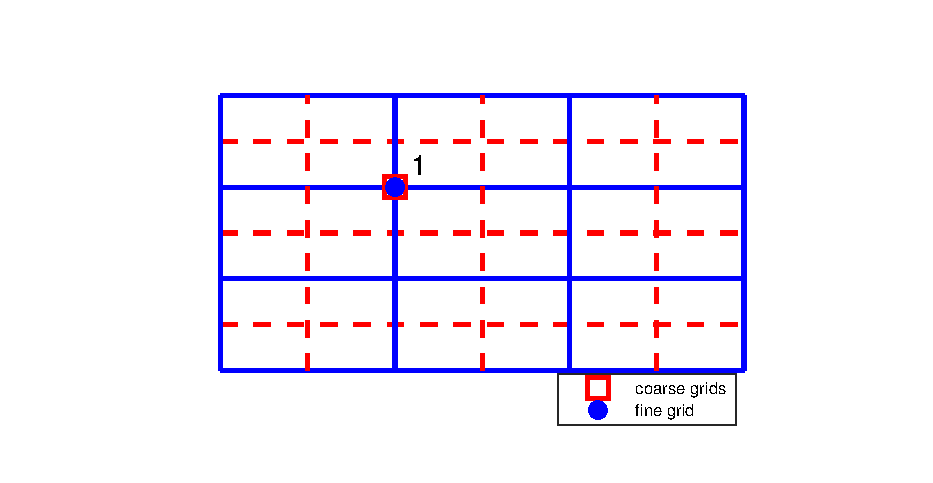
\includegraphics[width=0.24\textwidth,trim={1.8cm 0.8cm 1.4cm 1.2cm}, clip]{interpolation1.eps}
	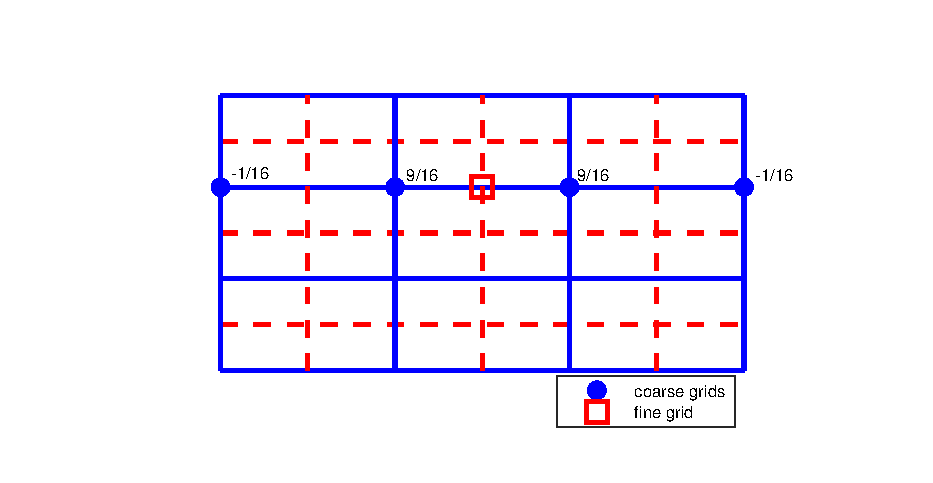
\includegraphics[width=0.24\textwidth,trim={1.8cm 0.8cm 1.4cm 1.2cm}, clip]{interpolation2.eps}
	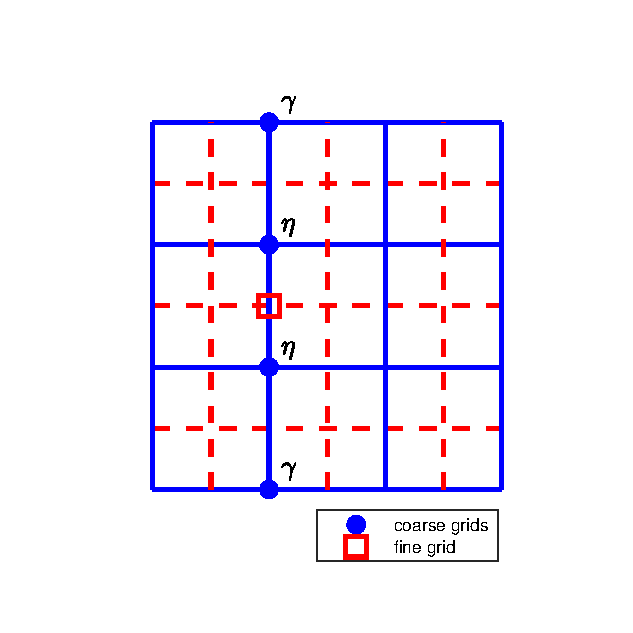
\includegraphics[width=0.24\textwidth,trim={1.8cm 0.8cm 1.4cm 1.2cm}, clip]{interpolation3.eps}
	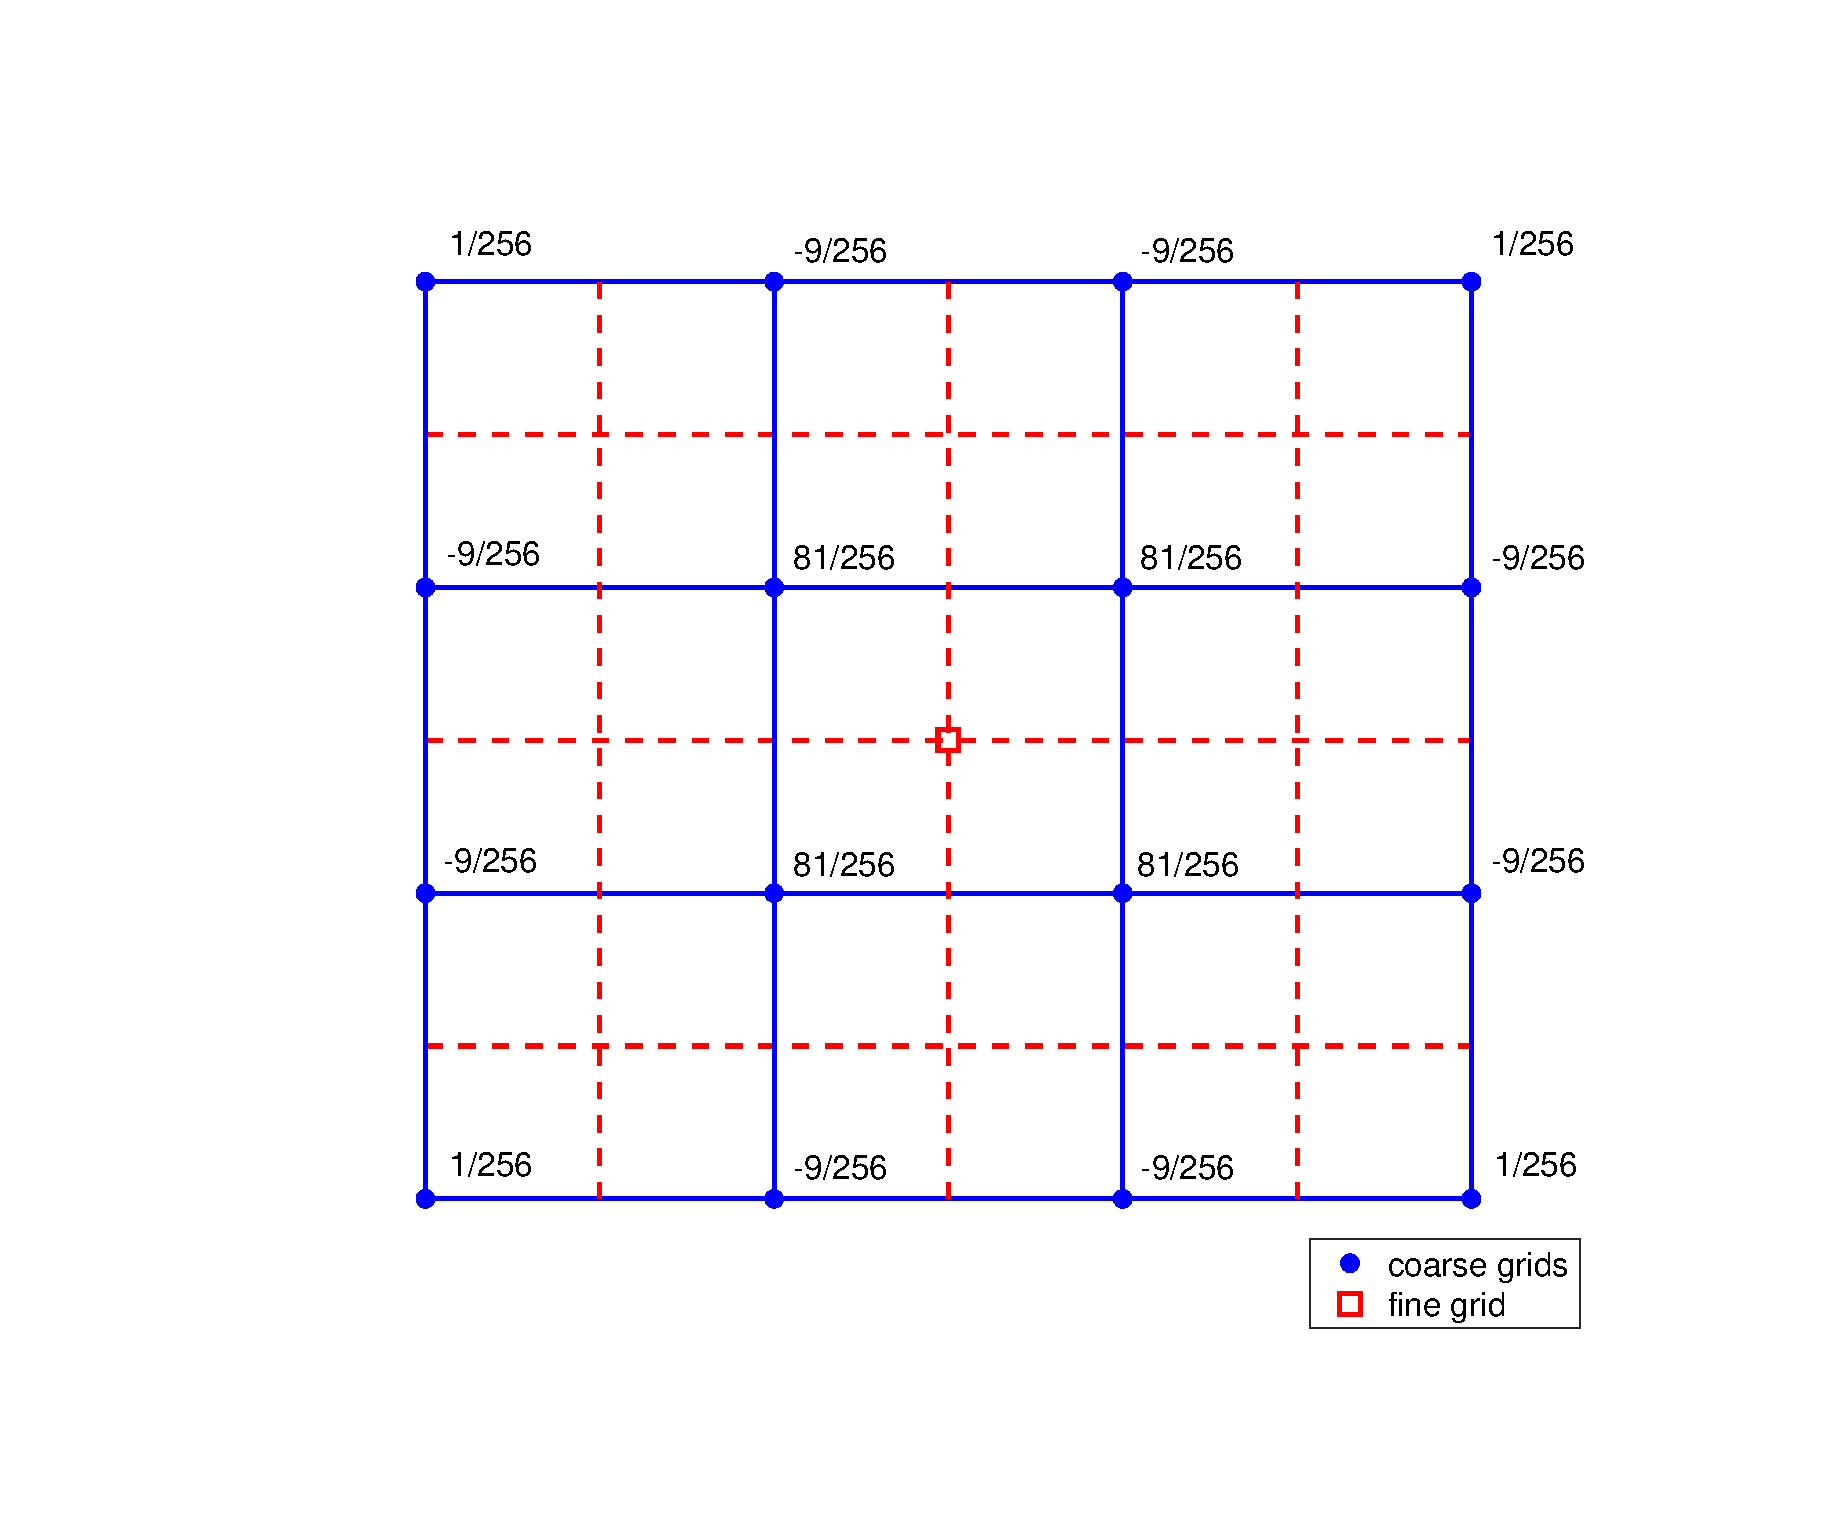
\includegraphics[width=0.24\textwidth,trim={1.8cm 0.8cm 1.4cm 1.2cm}, clip]{interpolation4.eps}
	\caption{The sketch for the stencils of fourth order interpolation operator ${\bf P}$ in two dimensions with parameters $\gamma = -\frac{1}{16}$, $\eta = \frac{9}{16}$, $\mu = 1$, $\alpha = \frac{1}{256}$, $\beta = -\frac{9}{256}$ and $\theta = \frac{81}{256}$. }\label{interpolation}
\end{figure}
\begin{figure}[htbp]
	\centering
	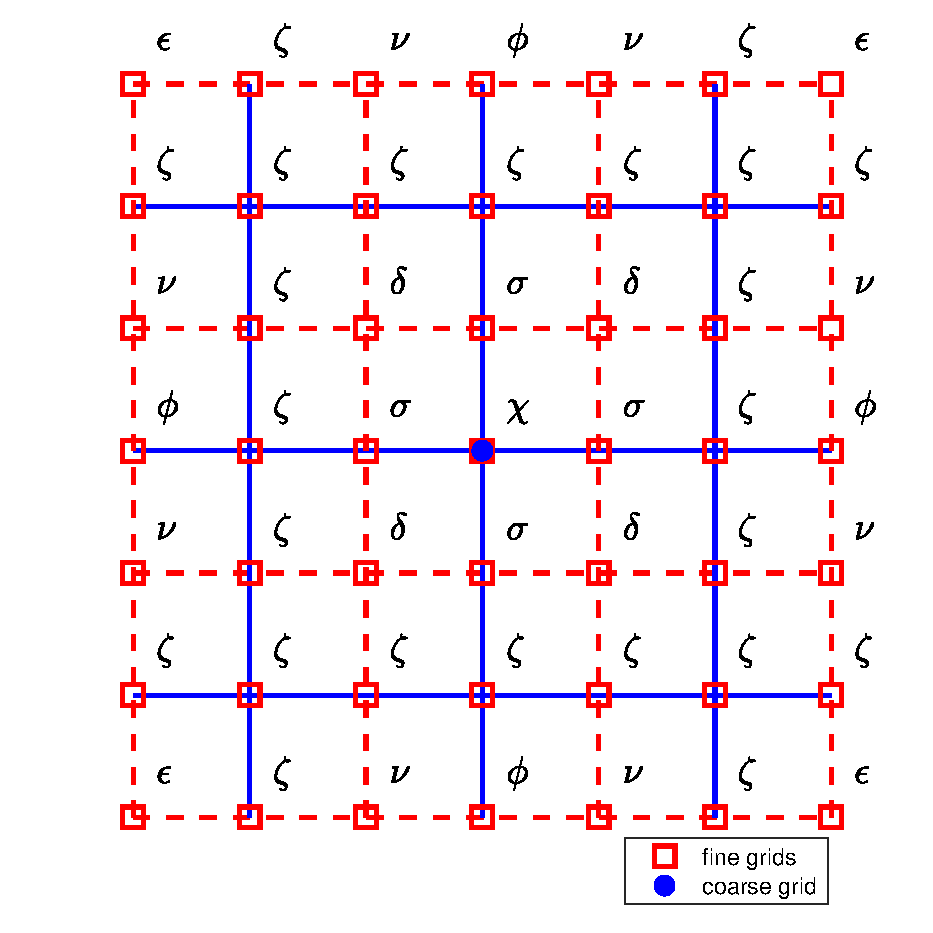
\includegraphics[width=0.6\textwidth]{restriction.eps}
	\caption{The sketch for the stencil of fourth order restriction operator ${\bf R}$ in two dimensions with parameters $\epsilon = \frac{1}{1024}$, $\nu = -\frac{9}{1024}$, $\phi = -\frac{16}{1024}$, $\delta = \frac{81}{1024}$, $\sigma = \frac{144}{1024}$, $\chi = \frac{256}{1024}$ and $\zeta = 0$.}\label{restriction}
\end{figure}

%To proceed with the interface conditions (\ref{interface_cond}), we firstly introduce scaled interpolation and restriction operators
%\[\wt{\mathcal{P}} = (\mathcal{J}^h_\Gamma \bm{\Lambda}^h)^{-\frac{1}{2}}\mathcal{P}(\mathcal{J}^{2h}_\Gamma \bm{\Lambda}^{2h})^{\frac{1}{2}},\ \ \ \ \wt{\mathcal{R}} =  (\mathcal{J}^{2h}_\Gamma \bm{\Lambda}^{2h})^{-\frac{1}{2}}\mathcal{R}(\mathcal{J}^{h}_\Gamma \bm{\Lambda}^h)^{\frac{1}{2}}.\]
%Here, both $\bm{\Lambda}^{h}$ and $\mathcal{R}$ are $3n_1^hn_2^hn_3^h\times 3n_1^hn_2^hn_3^h$ matrices, both $\bm{\Lambda}^{2h}$ and $\mathcal{P}$ are $3n_1^{2h}n_2^{2h}n_3^{2h}\times 3n_1^{2h}n_2^{2h}n_3^{2h}$ matrics, and they have the following structures
%\begin{align}\label{iandr}
%\mathcal{P} = \left(\begin{array}{ccc}
%{\bf P}& ~  & ~ \\
%~ & {\bf P} & ~ \\
%~ &~  &{\bf P}\end{array}\right),\ \ \mathcal{R} = \left(\begin{array}{ccc}
%{\bf R}& ~  & ~ \\
%~ & {\bf R} & ~ \\
%~ &~  &{\bf R}\end{array}\right),
%\end{align}
%%where $\bf P$ is a $n_1^{2h}n_2^{2h}n_3^{2h}\times n_1^{2h}n_2^{2h}n_3^{2h}$ matrix which has stencils as in Figure \ref{interpolation} and $\bf R$ is a $n_1^hn_2^hn_3^h\times n_1^hn_2^hn_3^h$ matrix with a stencil as in Figure \ref{restriction}
%%. And
%\begin{align}
%\bm{\Lambda}^h = \left(\begin{array}{ccc}
%\Lambda^h& ~  & ~ \\
%~ & \Lambda^h & ~ \\
%~ &~  &\Lambda^h\end{array}\right), \ \ \bm{\Lambda}^{2h} = \left(\begin{array}{ccc}
%\Lambda^{2h}& ~  & ~ \\
%~ & \Lambda^{2h} & ~ \\
%~ &~  &\Lambda^{2h}\end{array}\right),
%\end{align}
%where $\Lambda^{2h}$ is a $n_1^{2h}n_2^{2h}n_3^{2h}\times n_1^{2h}n_2^{2h}n_3^{2h}$ diagonal matrix and its diagonal value is $|\nabla_x^c r^{(3)}|$ evaluated at the coarse grid points on interface $\Gamma$; $\Lambda^{h}$ is a $n_1^{h}n_2^{h}n_3^{h}\times n_1^{h}n_2^{h}n_3^{h}$ diagonal matrix with diagonal value to be  $|\nabla_x^f r^{(3)}|$ evaluated at the fine grid points on interface $\Gamma$.


%Now, we are ready to work on continuous interface conditions (\ref{interface_cond}). In the discrete sense,  the grid functions ${\bf f}$ and ${\bf c}$ are coupled through interface conditions,
%\begin{equation}\label{continuous_sol}
%{\bf f}_{\Gamma} = \wt{\mathcal{P}}({\bf c}_{\Gamma}),
%\end{equation}
%which imposes the continuity of the solution at the interface $\Gamma$



